\chapter{Аналитическая часть}
%<пишем про тему и все, связанное с ней>
%➢ аналитический раздел:
%○ анализ существующих решений;
%○ уточнение требовании и формулировка ограничений предметной области;
%○ анализ баз данных по модели хранения данных;

\section{Анализ предметной области}
Авиаперелёты являются неотъемлимой частью современной жизни, в связи с этим появляется спрос на их отслеживание. Авиакомпании открывают рейсы, в последствии на которые люди покупают билеты. Для клиентов авиакомпании важно знать статус рейса, то есть будет ли рейс задержан или его перенесли, или вовсе отменили. Отслеживание перелётов подразумевает, что клиенту будет предоставлена информация о том, когда и где будет рейс, а также информация об изменеиях его расписания.

\section{Сравнительный анализ существующих конкурентов}
В таблице~\ref{table:competitors} представлен анализ существующих конкурентов.
\begin{table}[H]
	\caption{Конкуренты}
	\begin{tabularx}{\textwidth}{
			| >{\centering\arraybackslash}X
			| >{\centering\arraybackslash}X
			| >{\centering\arraybackslash}X
			| >{\centering\arraybackslash}X |
		}
		\hline
		Решение & Оповещение о полёте & Информация о задержках & Просмотр рейсов\\
		\hline
		Wanderlog & - & + & +\\
		\hline
		FlightStats & - & - & +\\
		\hline
		Flightradar24 & - & + & +\\
		\hline
	\end{tabularx}
	\label{table:competitors}
\end{table}

Из таблицы~\ref{table:competitors} видно, что представленные конкуренты не имеют функции оповещения пользователя о полёте.

\section{Формулировка требований к разрабатываемой базе данных и приложению}
База данных должна хранить информацию о пользователях, отслеживаемых ими рейсах, и о самих рейсах. Также информация в базе данных не должна быть противоречивой. Приложение должно предоставлять возможность просмотра рейсов и возможность отслеживания выбранного рейса.

\section{Формализация и описание информации, подлежащей хранению в проектируемой базе данных}
База данных должна хранить информацию о пользователях, аэропортах, выходах на посадку, моделях самолётов, самолётах, рейсах, маршрутов рейсов, о том какие рейсы отслеживает пользователь и о уведомлениях, которые необходимо отправить пользователю.

Хранимая информация о пользователе:
\begin{itemize}
	\item адрес электронной почты;
	\item пароль.
\end{itemize}

Хранимая информация об аэропорте:
\begin{itemize}
	\item IATA код --- код используемый для обозначения аэропорта;
	\item название аэропорта;
	\item город, в котором расположен аэропорт;
	\item страна, в которой расположен аэропорт.
\end{itemize}

Хранимая информация о выходе на посадку:
\begin{itemize}
	\item информация об аэропорте, в котором расположен выход;
	\item номер выхода.
\end{itemize}

Хранимая информация о модели самолёта:
\begin{itemize}
	\item производитель;
	\item название модели;
	\item масса;
	\item максимальная высота, на которую может подняться самолёт;
	\item максимальная скорость, которую может развить самолёт.
\end{itemize}

Хранимая информация о самолёте:
\begin{itemize}
	\item информация о модели самолёта;
	\item регистрационный номер --- уникальный номер, который выдаёт государство, где зарегистрирован самолёт;
	\item бортовой номер --- уникальный номер, присваиваемый производителем при выпуске;
	\item сколько миль пролетел самолёт.
\end{itemize}

Хранимая информация о рейсе:
\begin{itemize}
	\item самолёт, который выполняет рейс;
	\item запланированная дата вылета;
	\item запланированная дата прилёта;
	\item фактическая дата вылета;
	\item фактическая дата прилёта;
	\item статус;
	\item план.
\end{itemize}

Хранимая информация о маршруте рейса:
\begin{itemize}
	\item аэропорт вылета;
	\item аэропорт прилёта.
\end{itemize}

Хранимая информация о рейсах, интересующих пользователя:
\begin{itemize}
	\item информация о пользователе;
	\item информация о рейсе.
%	\item информация за сколько прислать уведомление.
\end{itemize}

Хранимая информация о уведомлениях пользователя:
\begin{itemize}
	\item информация о содержании уведомления;
	\item когда создано уведомление;
	\item когда отправить уведомление;
	\item состояние уведомления.
	%	\item информация за сколько прислать уведомление.
\end{itemize}

Связи между описанными объектами бд:
\begin{itemize}
	\item один аэропорт может содержать несколько выходов на посадку;
	\item одна модель самолёта может соответствовать нескольким самолётам;
	\item один самолёт может выполнять несколько рейсов;
	\item один маршрут может использоваться несколькими рейсами;
	\item один пользователь может отслеживать несколько рейсов;
	\item один рейс может отслеживаться несколькими пользователями;
	\item для одного пользователя может быть создано несколько уведомлений.
\end{itemize}

\section{Проведенный анализ существующих баз данных на основе формализации данных}
По модели хранения данных бд подразделяются на
\begin{itemize}
	\item иерархические
	\item сетевые
	\item реляционные
	\item нереляционные
\end{itemize}

Сущности имеют атрибуты, также необходимо поддерживать связь между сущностями, также необходимо обеспечить безопасность со стороны базы данных Таким образом была выбрана реляционная база данных.

\section{ER-диаграмма сущностей проектируемой базы данных в нотации Чена}
На рисунке~\ref{fig:er} представлена ER-диаграмма сущностей проектируемой базы данных.
\begin{figure}[H]
	\centering
	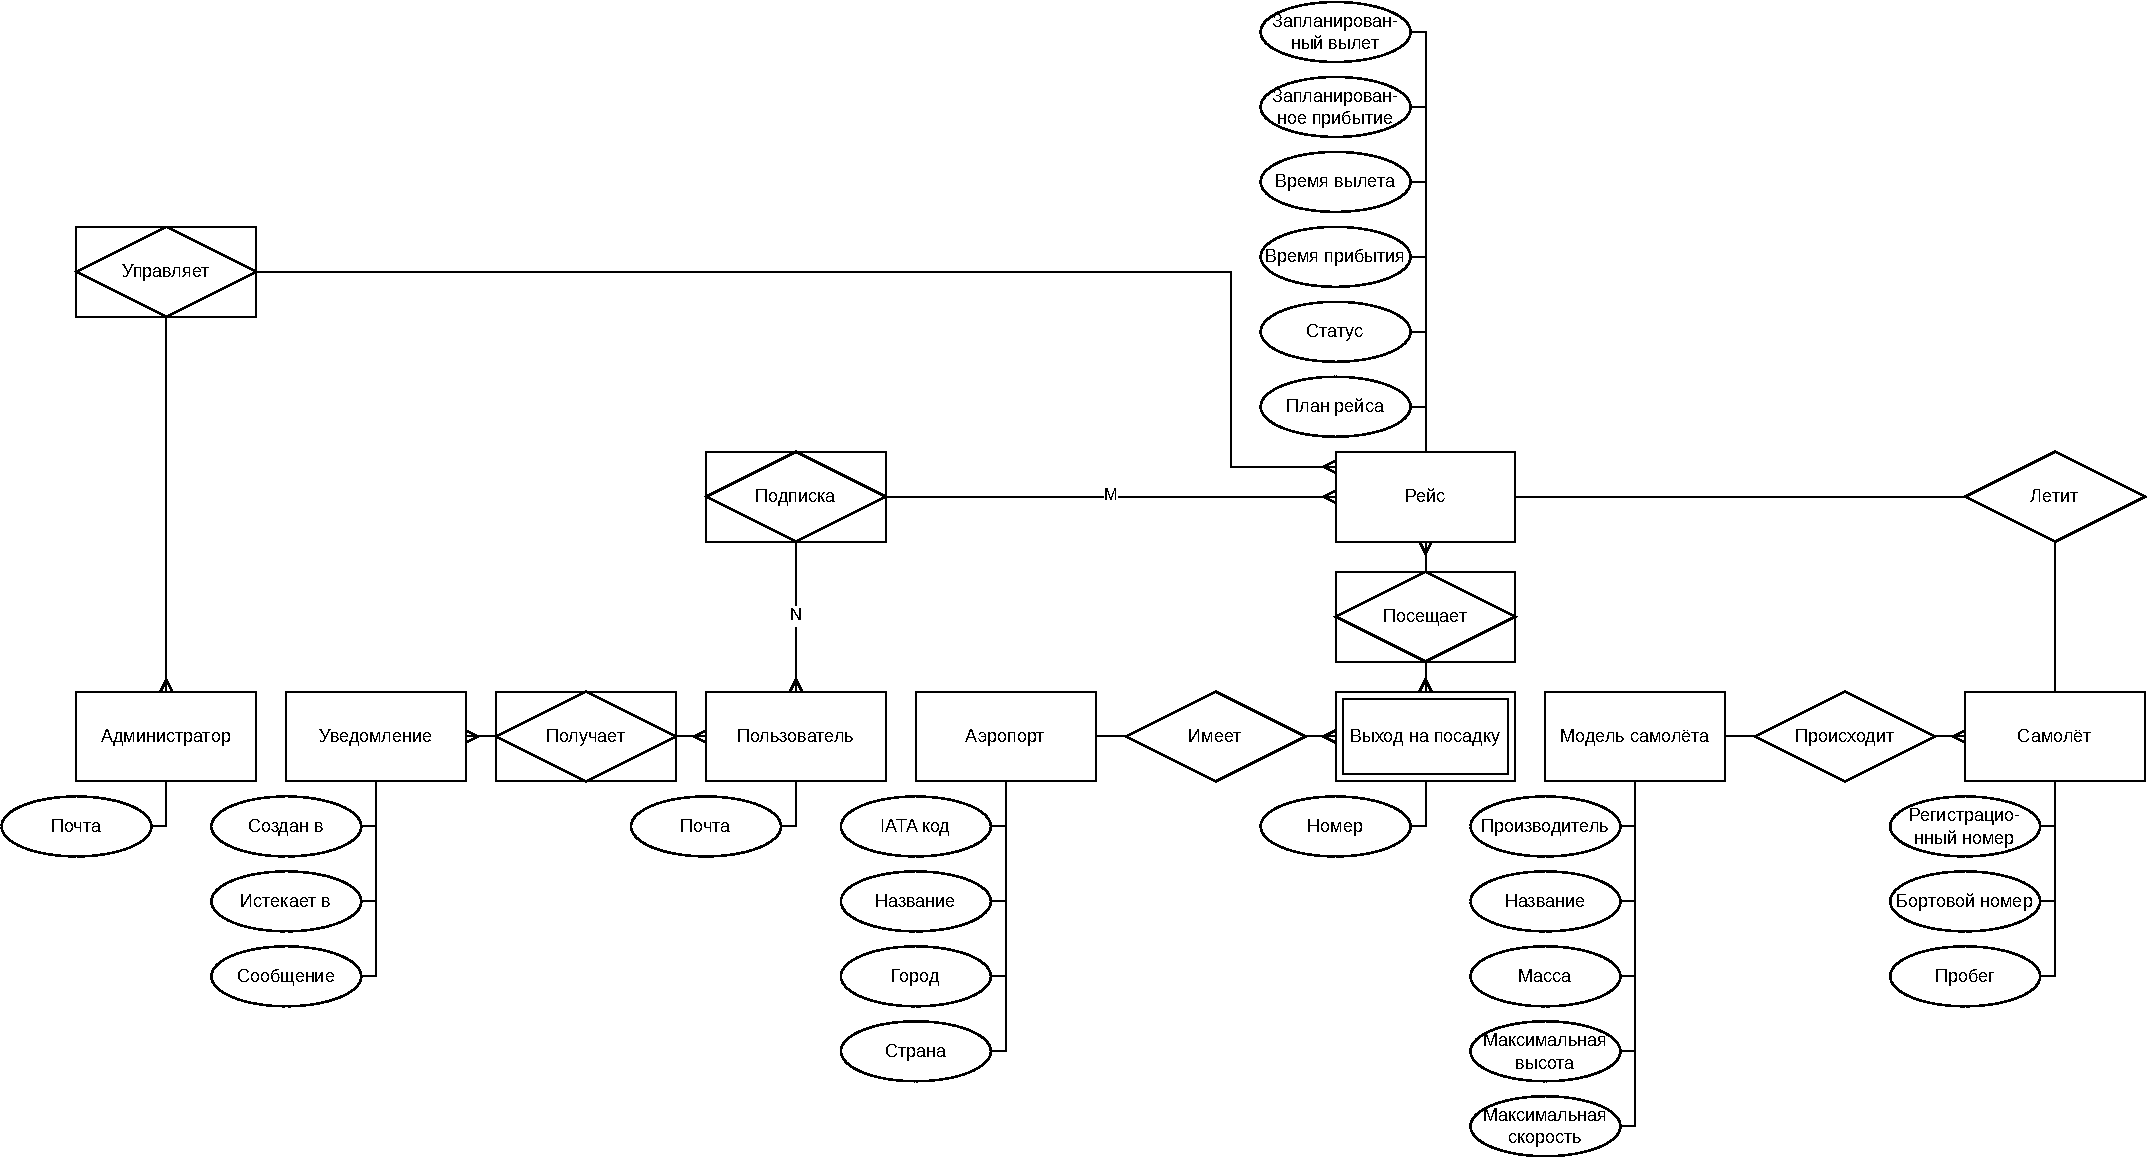
\includegraphics[width=1.0\columnwidth, angle=90, height=0.9\textheight]{diags/er.pdf}
	\caption{Диаграмма вариантов использования}
	\label{fig:er}
\end{figure}

\section{Формализация и описание пользователей проектируемого приложения к базе данных}
Пользователи приложения подразделяются на администратора, обычного пользователя и авторизованного пользователя. Администратор управляет информацией о полётах. Все пользователи могут просматривать информацию о рейсах, а авторизованный пользователь может отслеживать изменения интересующих рейсов.

\section{Диаграмма вариантов использования}
На рисунке~\ref{fig:usecase} представлена диаграмма вариантов использования приложения.

\begin{figure}[H]
	\centering
	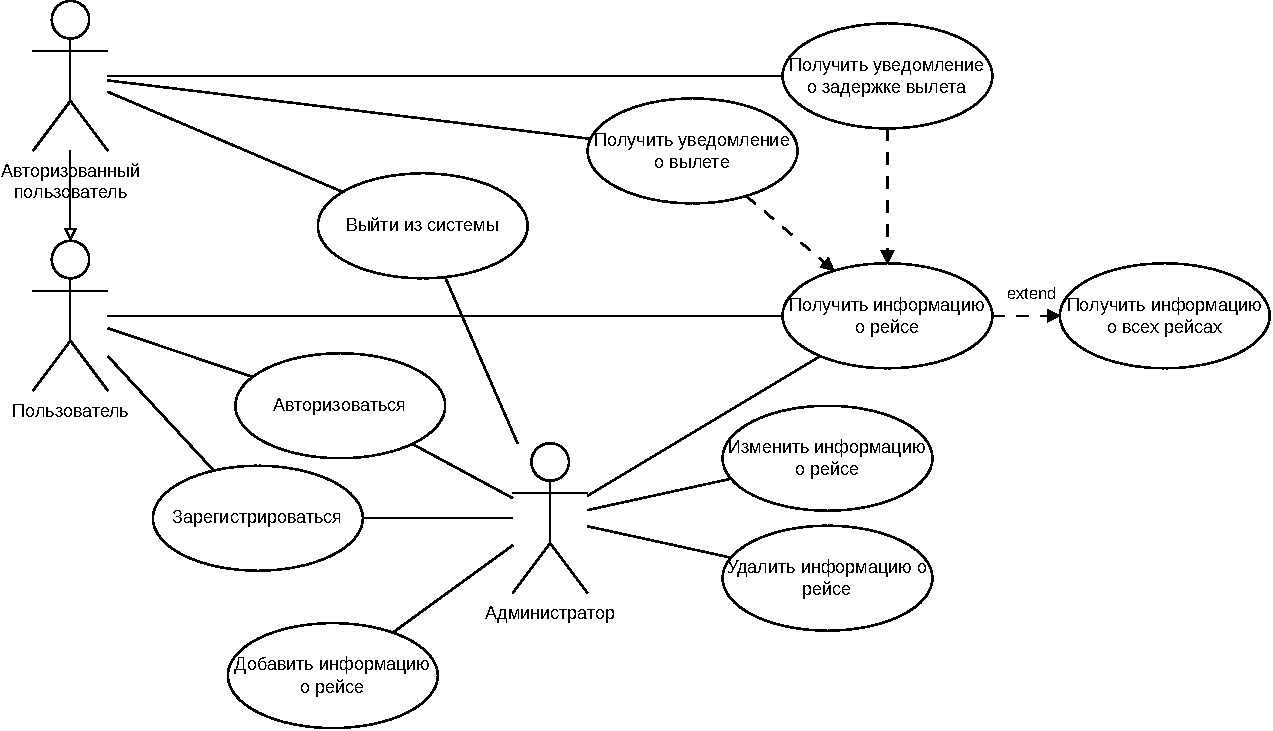
\includegraphics[height=0.35\textheight]{diags/usecase.pdf}
	\caption{Диаграмма вариантов использования приложения}
	\label{fig:usecase}
\end{figure}

\clearpage